\section{Interfaz Web}

Se desarrolló una interfaz web utilizando el framework Astro, que se encuentra alojada por el momento de manera local, este consulta un endpoint construido en Java que se conecta a su vez con la base de datos PostgreSQL, que se aloja en la nube de Render. 

\subsection{ProductoDAO}

Es una clase en Java que permite realizar operaciones de acceso a datos para la entidad "Producto". Esta clase se encarga de interactuar con la base de datos para realizar operaciones como insertar, actualizar, eliminar y consultar productos.

\subsection{Endpoints}

Se creó el endpoint \texttt{/productos} que permitirá realizar operaciones CRUD (Crear, Leer, Actualizar, Eliminar) sobre los productos almacenados en la base de datos. Por ahora solo se ha implementado la funcionalidad de lectura, que permite obtener la lista de productos disponibles.

\subsection{Interfaz de Usuario}

La interfaz de usuario se diseñó para ser intuitiva y fácil de usar. Se muestra una lista de productos con sus respectivos detalles, como nombre, descripción y precio.

\begin{figure}[H]
    \centering
    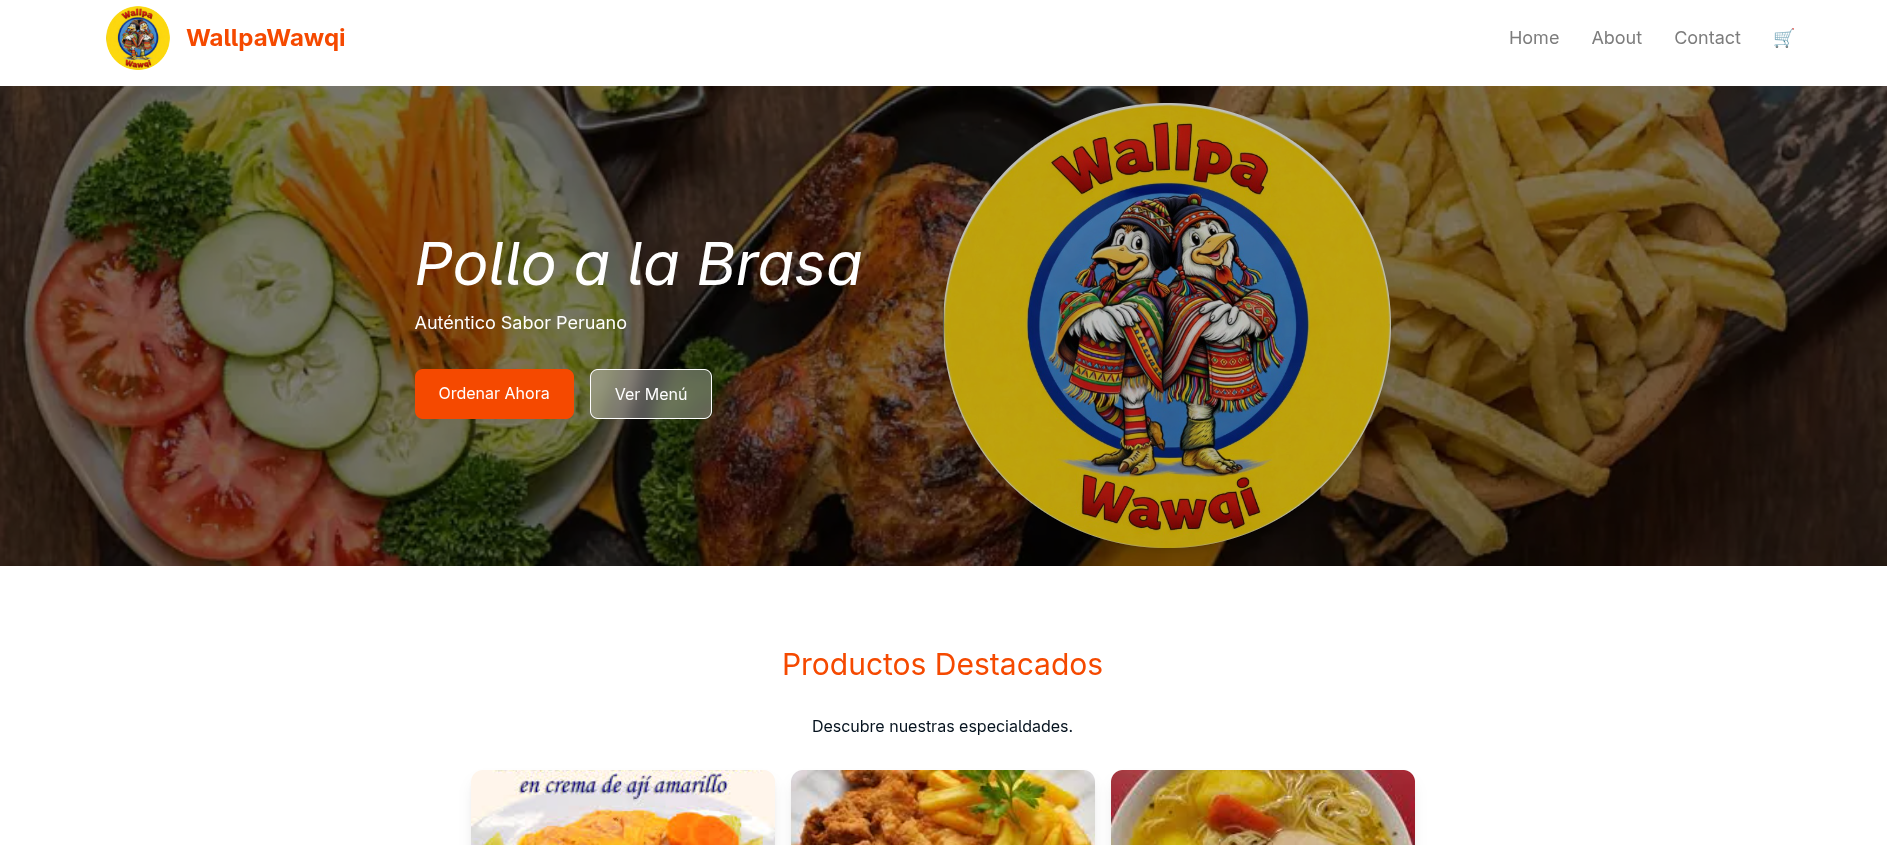
\includegraphics[width=1\textwidth]{assets/front_1.png}
    \caption{Interfaz web, Hero o parte principal.}

\end{figure}

\begin{figure}[H]
    \centering
    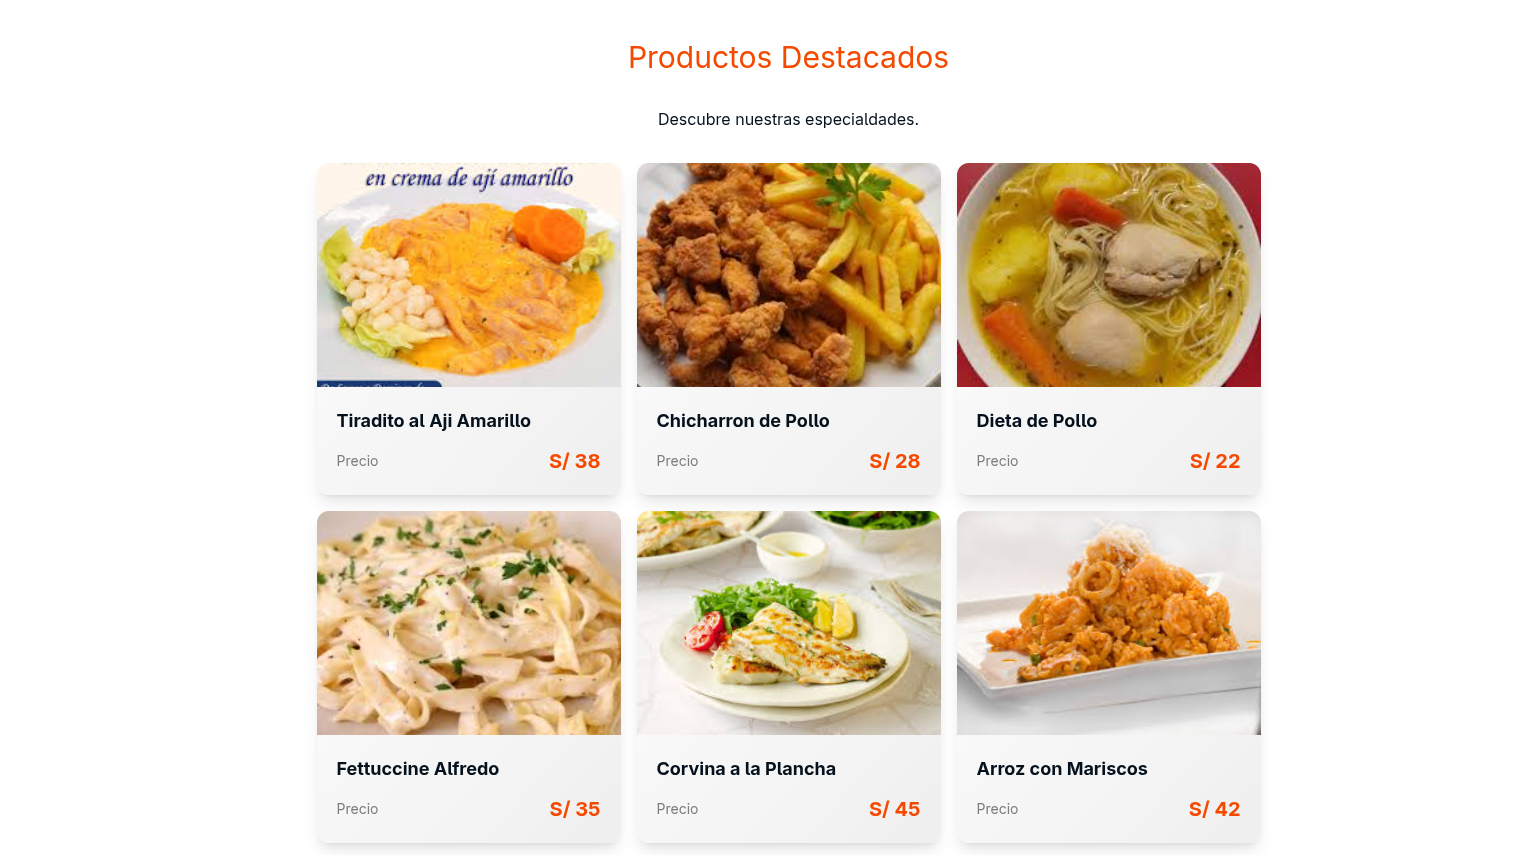
\includegraphics[width=1\textwidth]{assets/front_2.png}
    \caption{Interfaz web, sección de productos.}
\end{figure}